\documentclass{article}
\usepackage{tikz}

\begin{document}

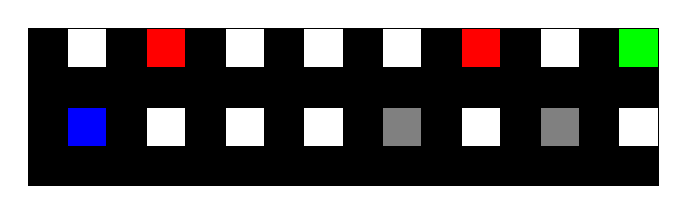
\begin{tikzpicture}[scale=0.5]
    \draw[fill=black] (0,0) rectangle (16,4);
    \draw[fill=white] (1,1) rectangle (2,2);
    \draw[fill=white] (3,1) rectangle (4,2);
    \draw[fill=white] (5,1) rectangle (6,2);
    \draw[fill=white] (7,1) rectangle (8,2);
    \draw[fill=white] (9,1) rectangle (10,2);
    \draw[fill=white] (11,1) rectangle (12,2);
    \draw[fill=white] (13,1) rectangle (14,2);
    \draw[fill=white] (15,1) rectangle (16,2);
    \draw[fill=white] (1,3) rectangle (2,4);
    \draw[fill=white] (3,3) rectangle (4,4);
    \draw[fill=white] (5,3) rectangle (6,4);
    \draw[fill=white] (7,3) rectangle (8,4);
    \draw[fill=white] (9,3) rectangle (10,4);
    \draw[fill=white] (11,3) rectangle (12,4);
    \draw[fill=white] (13,3) rectangle (14,4);
    \draw[fill=white] (15,3) rectangle (16,4);
    
    \draw[fill=blue] (1,1) rectangle (2,2);
    \draw[fill=red] (3,3) rectangle (4,4);
    \draw[fill=red] (11,3) rectangle (12,4);
    \draw[fill=gray] (9,1) rectangle (10,2);
    \draw[fill=gray] (13,1) rectangle (14,2);
    \draw[fill=green] (15,3) rectangle (16,4);
\end{tikzpicture}

Illustration of the passageway environment. The agent moves within the black walls, starting from the blue tile, it must reach the red switches to open the gray doors, and reach the final green position.